\documentclass{../../slides-style}

\slidetitle{Модульное тестирование}{}

\begin{document}
    
    \begin{frame}[plain]
        \titlepage
    \end{frame}

    \section{Введение}

    \begin{frame}
        \frametitle{Модульное тестирование: зачем?}
        \begin{enumerate}
            \item Любая программа содержит ошибки
            \item Если программа не содержит ошибок, их содержит алгоритм, который реализует эта программа
            \item Если ни программа, ни алгоритм ошибок не содержат, такая программа даром никому не нужна
        \end{enumerate}
    \end{frame}

    \section{Пример}

    \begin{frame}
        \frametitle{Пример}
        Консольный калькулятор, складывающий два двузначных числа
        \begin{itemize}
            \item Называется adder
            \item Ввод числа заканчивается нажатием на \textit{Enter}
            \item Программа должна вывести сумму после ввода второго числа
        \end{itemize}
        \begin{textblock}{5}(5,2)
            \attribution{C. Kaner, Testing Computer Software}
        \end{textblock}
    \end{frame}

    \begin{frame}
        \frametitle{Смоук-тест}
        \begin{center}
            \begin{tabu} {| X[0.6 l p] | X[1 l p] |}
                \tabucline-
                \everyrow{\tabucline-}
                \textbf{Что делаем}                             & \textbf{Что происходит}                                                            \\
                Вводим \textit{adder} и жмём на \textit{Enter}  & Экран мигает, внизу появляется знак вопроса                                        \\
                Нажимаем 2                                      & За знаком вопроса появляется цифра 2                                               \\
                Нажимаем \textit{Enter}                         & В следующей строке появляется знак вопроса                                         \\
                Нажимаем 3                                      & За вторым знаком вопроса появляется цифра 3                                        \\
                Нажимаем \textit{Enter}                         & В третьей строке появляется 5, несколькими строками ниже --- ещё один знак вопроса
            \end{tabu}
        \end{center}
    \end{frame}

    \begin{frame}
        \frametitle{Выявленные проблемы}
        \begin{itemize}
            \item Нет названия программы на экране, может, мы запустили не то
            \item Нет никаких инструкций, пользователь без идей, что делать
            \item Непонятно, как выйти
        \end{itemize}
    \end{frame}

    \begin{frame}
        \frametitle{План дальнейших тестов}
        \begin{scriptsize}
            \begin{center}
                \begin{tabu} {| X[2 l p] | X[2 l p] | X[7 l p] |}
                    \tabucline-
                    \everyrow{\tabucline-}
                    \textbf{Ввод}  & \textbf{Ожидаемый результат}  & \textbf{Замечания}                                                      \\
                    99 + 99        & 198                           & Пара наибольших допустимых чисел                                        \\
                    -99 + -99      & -198                          & Отрицательные числа, почему нет?                                        \\
                    99 + -14       & 85                            & Большое первое число может влиять на интерпретацию второго              \\
                    -38 + 99       & 61                            & Отрицательное плюс положительное                                        \\
                    56 + 99        & 155                           & Большое второе число может повлиять на интерпретацию первого            \\
                    9 + 9          & 18                            & Два наибольших числа из одной цифры                                     \\
                    0 + 0          & 0                             & Программы часто не работают на нулях                                    \\
                    0 + 23         & 23                            & 0 --- подозрительная штука, его надо проверить и как первое слагаемое,  \\
                    -78 + 0        & -78                           & и как второе
                \end{tabu}
            \end{center}
        \end{scriptsize}
    \end{frame}

    \begin{frame}
        \frametitle{План дальнейших тестов (2)}
        \begin{scriptsize}
            \begin{center}
                \begin{tabu} {| X[2 l p] | X[7 l p] |}
                    \tabucline-
                    \everyrow{\tabucline-}
                    \textbf{Ввод}                   & \textbf{Замечания}                                                 \\
                    100 + 100                       & Поведение сразу за диапазоном допустимых значений                  \\
                    \textit{Enter} + \textit{Enter} & Что будет, если данные не вводить вообще                           \\
                    123456 + 0                      & Введём побольше цифр                                               \\
                    1.2 + 5                         & Вещественные числа, пользователь может решить, что так можно       \\
                    A + b                           & Недопустимые символы, что будет?                                   \\
                    Ctrl-A, Ctrl-D, F1, Esc         & Управляющие клавиши часто источник проблем в консольных программах \\
                \end{tabu}
            \end{center}
        \end{scriptsize}
    \end{frame}

    \begin{frame}
        \frametitle{Ещё больше тестов!}
        \begin{itemize}
            \item Внутреннее хранение данных --- двузначные числа могут хранить в \textbf{byte}
            \begin{itemize}
                \item 99 + 99, этот случай покрыли
            \end{itemize}
            \item Кодовая страница ввода: символы '/', '0', '9' и ':'
            \begin{itemize}
                \item Программист может напутать со строгостью неравенства при проверке
                \item Не надо вводить A + b, достаточно граничные символы
            \end{itemize}
        \end{itemize}
    \end{frame}

    \begin{frame}
        \frametitle{Информация к размышлению}
        \begin{itemize}
            \item Программа из сотни строк может иметь $10^{18}$ путей исполнения
            \begin{itemize}
                \item Времени жизни вселенной не хватило бы, чтобы их покрыть
            \end{itemize}
            \item После передачи на тестирование в программах в среднем от 1 до 3 ошибок на 100 строк кода
            \item В процессе разработки --- 1.5 ошибок на 1 строку кода (!)
            \item Если для исправления ошибки надо изменить не более 10 операторов, с первого раза это делают правильно в 50\% случаев
            \item Если для исправления ошибки надо изменить не более 50 операторов, с первого раза это делают правильно в 20\% случаев
        \end{itemize}
    \end{frame}

    \section{Модульные тесты}

    \begin{frame}
        \frametitle{Модульные тесты}
        \begin{itemize}
            \item Тестирование отдельного класса
            \item Проверяют внешнее поведение класса
            \item Полностью автоматические
            \item Направлены на поиск ошибок в конкретном методе
            \item Не влияют на функциональность системы и не поставляются пользователю
        \end{itemize}
    \end{frame}

    \begin{frame}
        \frametitle{Почему модульные тесты полезны}
        \begin{itemize}
            \item Помогают искать ошибки
            \begin{itemize}
                \item Особо эффективны, если налажен процесс Continuous Integration
            \end{itemize}
            \item Облегчают изменение программы
            \begin{itemize}
                \item Помогают при рефакторинге
            \end{itemize}
            \item Тесты --- документация к коду
            \item Помогают улучшить архитектуру
            \item НЕ доказывают отсутствие ошибок в программе
        \end{itemize}
    \end{frame}

    \begin{frame}
        \frametitle{``Базовые'' библиотеки модульного тестирования}
        \begin{itemize}
            \item JVM: JUnit 5 (хотя JUnit 4 тоже довольно популярен)
            \begin{itemize}
                \item Kent Beck и Erich Gamma, аж 1997 год
                \item Самая популярная библиотека для JVM
            \end{itemize}
            \item С++: Google Test, Boost.Test, CTest, Qt Test
            \item Python: PyTest
            \item .NET: NUnit, xUnit, Microsoft Unit Test Framework
        \end{itemize}
    \end{frame}

    \begin{frame}
        \frametitle{Пример, юнит-тесты в C\#}
        \begin{itemize}
            \item Для тех, кто всё пропустил: \url{https://msdn.microsoft.com/en-us/library/hh694602.aspx\#BKMK\_Quick\_starts}
        \end{itemize}
    \end{frame}

    \begin{frame}[fragile]
        \frametitle{Data-driven-тесты}
            \begin{minted}{csharp}
[TestCase(12, 3, 4)]
[TestCase(12, 2, 6)]
public void DivideTest(int n, int d, int q)
{
    Assert.AreEqual(q, n / d);
}
        \end{minted}
        \vspace{3mm}
        Или даже
        \begin{minted}{csharp}
[TestCase(12, 3, ExpectedResult = 4)]
[TestCase(12, 2, ExpectedResult = 6)]
public int DivideTest(int n, int d)
{
    return n / d;
}
        \end{minted}
    \end{frame}

    \begin{frame}
        \frametitle{Best practices (1)}
        \begin{itemize}
            \item Чёткое разделение на три фазы (Arrange-Act-Assert)
            \begin{itemize}
                \item Настройка тестового окружения и тестируемой системы (SUT)
                \item Выполнение действия
                \item Проверка результатов
            \end{itemize}
            \item Именование тестов: ``в таких-то условиях should происходить то-то''
            \begin{itemize}
                \item \url{https://stackoverflow.com/questions/155436/unit-test-naming-best-practices}
            \end{itemize}
            \item Модульные тесты тестируют один модуль
            \begin{itemize}
                \item Mock-объекты
            \end{itemize}
        \end{itemize}
    \end{frame}

    \begin{frame}
        \frametitle{Best practices (2)}
        \begin{itemize}
            \item Независимость тестов
            \begin{itemize}
                \item Желательно, чтобы поломка одного куска функциональности ломала один тест
                \item Подчищать за собой данные, не использовать глобальное состояние
                \item Тесты могут исполняться параллельно!
            \end{itemize}
            \item Тесты должны работать быстро
            \begin{itemize}
                \item И запускаться после каждой сборки
                \begin{itemize}
                    \item Continuous Integration!
                \end{itemize}
            \end{itemize}
            \item Тестов должно быть много
            \begin{itemize}
                \item Следить за Code coverage
            \end{itemize}
            \item Каждый тест должен проверять конкретный тестовый сценарий
            \begin{itemize}
                \item Исключить случайность, не использовать try/catch в тестах
            \end{itemize}
            \item Test-driven development
        \end{itemize}
    \end{frame}

    \section{Мок-объекты}

    \begin{frame}
        \frametitle{Mock-объекты}
        \begin{itemize}
            \item Объекты-заглушки, подставляемые вместо реальных
        \end{itemize}
        \begin{center}
            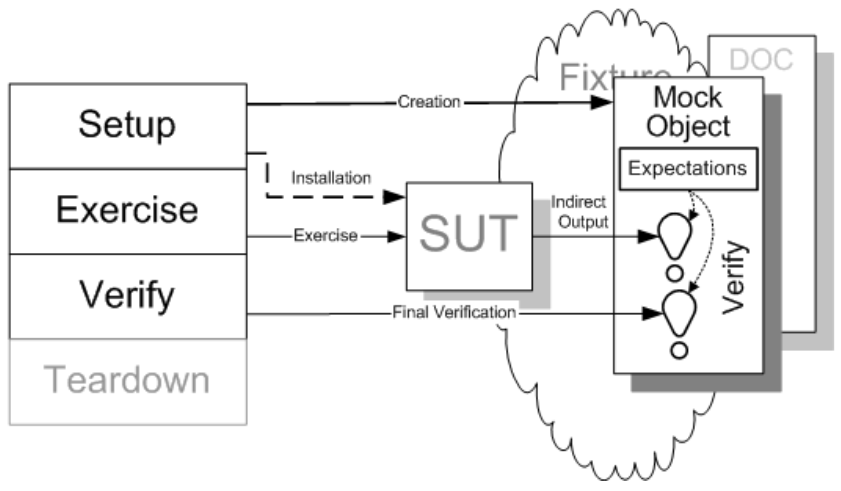
\includegraphics[width=0.6\textwidth]{mock.png}
            \attribution{http://xunitpatterns.com}
        \end{center}
    \end{frame}

    \begin{frame}
        \frametitle{Когда использовать}
        \begin{itemize}
            \item Когда тестируемый модуль вызывает много чего ещё --- непонятно, что сломалось, если тест не прошёл
            \item Когда выполнение реальной операции долго или небезопасно
            \item Когда есть механизм внедрения mock-объекта --- dependency injection
            \begin{itemize}
                \item Хороший код и так должен это делать
            \end{itemize}
        \end{itemize}
    \end{frame}

    \begin{frame}
        \frametitle{Библиотеки mock-объектов}
        \begin{itemize}
            \item JVM: Mockito, EasyMock
            \item C++: Google Test
            \item Python: unittest.mock
            \item .NET: Moq, NSubstitute
        \end{itemize}
    \end{frame}

    \begin{frame}[fragile]
        \frametitle{Пример, Mockito, классический тест}
        \begin{minted}{java}
@Test 
public void test() throws Exception {
    // Arrange
    var testee = new UnitToTest();
    var helper = new Helper();
    // Act
    testee.doSomething(helper);
    // Assert
    assertTrue(helper.somethingHappened());
}
        \end{minted}
    \end{frame}

    \begin{frame}[fragile]
        \frametitle{Пример, Mockito, тест с mock-объектом}
        \begin{minted}{java}
@Test
public void test() throws Exception {
    // Arrange, prepare behaviour
    var testee = new UnitToTest();
    Helper aMock = mock(Helper.class);
    when(aMock.isCalled()).thenReturn(true);
    // Act
    testee.doSomething(aMock);
    // Assert - verify interactions (optional)
    verify(aMock).isCalled();
}
        \end{minted}
    \end{frame}

    \section{Матчеры}

    \begin{frame}
        \frametitle{Матчеры}
        \begin{itemize}
            \item Писать Assert.AreEqual неудобно и не всегда типобезопасно
            \item Сейчас модна объектная модель условия, те самые Matchers (или Constraints)
            \begin{itemize}
                \item Пример (NUnit): \mintinline{csharp}|Assert.That(array, Has.Exactly(1).EqualTo(3));|
            \end{itemize}
            \item Библиотеки: Hamcrest (JUnit) / NHamcrest (NUnit)
            \item Многие библиотеки юнит-тестирования умеют что-то такое ``из коробки''
        \end{itemize}
    \end{frame}

    \section{Фаззинг}

    \begin{frame}[fragile]
        \frametitle{Property-driven testing, фаззинг}
        \begin{itemize}
            \item А пусть тестовая система сама генерирует данные на вход!
            \item Пример, FsCheck:
                \begin{small}
                    \begin{minted}{fsharp}
open FsCheck

let revRevIsOrig (xs:list<int>) = List.rev (List.rev xs) = xs

Check.Quick revRevIsOrig
// Ok, passed 100 tests.

let revIsOrig (xs:list<int>) = List.rev xs = xs

Check.Quick revIsOrig
// Falsifiable, after 2 tests (2 shrinks) (StdGen (338235241,296278002)):
// Original:
// [3; 0]
// Shrunk:
// [1; 0]
                    \end{minted}
                \end{small}
        \end{itemize}
    \end{frame}

    \section{UI-тестирование}

    \begin{frame}
        \frametitle{UI-тестирование}
        \begin{columns}
            \begin{column}{0.5\textwidth}
                \begin{itemize}
                    \item Есть ещё интеграционные тесты и UI-тесты
                    \item UI-тестирование: Selenium (Web), FlaUI (или White) и подобные штуки --- настольные приложения
                \end{itemize}
            \end{column}
            \begin{column}{0.5\textwidth}
                
\includegraphics[width=0.9\textwidth]{titanic.png}
                \attribution{Интернеты}
            \end{column}
        \end{columns}
    \end{frame}

\end{document}